\documentclass[12pt]{article}

\usepackage{amsmath, mathtools}
\usepackage{amsfonts}
\usepackage{amssymb}
\usepackage{graphicx}
\usepackage{colortbl}
\usepackage{xr}
\usepackage{hyperref}
\usepackage{longtable}
\usepackage{xfrac}
\usepackage{tabularx}
\usepackage{float}
\usepackage{booktabs}
\usepackage{caption}
\usepackage{pdflscape}
\usepackage{afterpage}

\usepackage[round]{natbib}

\hypersetup{
    bookmarks=true,         % show bookmarks bar?
    colorlinks=true,       % false: boxed links; true: colored links
    linkcolor=red,          % color of internal links (change box color with linkbordercolor)
    citecolor=green,        % color of links to bibliography
    filecolor=magenta,      % color of file links
    urlcolor=cyan           % color of external links
}

%% Comments

\usepackage{color}

\newif\ifcomments\commentstrue %displays comments
%\newif\ifcomments\commentsfalse %so that comments do not display

\ifcomments
\newcommand{\authornote}[3]{\textcolor{#1}{[#3 ---#2]}}
\newcommand{\todo}[1]{\textcolor{red}{[TODO: #1]}}
\else
\newcommand{\authornote}[3]{}
\newcommand{\todo}[1]{}
\fi

\newcommand{\wss}[1]{\authornote{blue}{SS}{#1}} 
\newcommand{\plt}[1]{\authornote{magenta}{TPLT}{#1}} %For explanation of the template
\newcommand{\an}[1]{\authornote{cyan}{Author}{#1}}

%% Common Parts

\newcommand{\progname}{Mechtronics Enigeering} % PUT YOUR PROGRAM NAME HERE
\newcommand{\authname}{Team 32, Wingman
\\ Edward He
\\ Erping Zhang
\\ Guangwei Tang
\\ Peng Cui
\\ Peihua Jin } % AUTHOR NAMES                  

\usepackage{hyperref}
    \hypersetup{colorlinks=true, linkcolor=blue, citecolor=blue, filecolor=blue,
                urlcolor=blue, unicode=false}
    \urlstyle{same}
                                


\title{Software Requirements Specification\\\progname}

\author{\authname}

\date{}

\begin{document}

\maketitle

\newpage
\pagenumbering{roman}

\tableofcontents

\newpage

\begin{table}[hp]
\caption{Revision History} \label{TblRevisionHistory}
\begin{tabularx}{\textwidth}{llX}
\toprule
\textbf{Date} & \textbf{Developer(s)} & \textbf{Change}\\
\midrule
2022-10-04 & Edward He, Erping Zhang & Revision 0\\
& Guangwei Tang, Peng Cui & \\
& Peihua Jin & \\
\bottomrule
\end{tabularx}
\end{table}

\newpage

\listoftables
\listoffigures

\newpage

\pagenumbering{arabic}

This document describes the requirements for \progname. The template for the Software
Requirements Specification (SRS) is a subset of the Volere
template~\cite{RobertsonAndRobertson2012}. If you make further modifications
to the template, you should explicitly state what modifications were made.

\begin{table}

\end{table}

\section{Project Drivers}

\subsection{The Purpose of the Project}
The purpose of the project is to build a mechatronics system called "SmartVault" that is able to assist user in finding their belongings in a given area. 
\subsection{The Purpose of the Document}
This document is intended to provide detailed set of requirements project SmartVault. The documentation will cover the functionality of the system and the requirements that the system is expected to fulfill. In addition to the function requirements of software system, non-functional requirements will also be included in this document. Any additional useful information for building the system is also covered and written in details. This document is used as a reference and guideline for the development of the system and is to ensure that the built system is fulfilling the necessary requirements and meeting the desired goals.
\subsection{The Stakeholders}

\subsubsection{The Client}
\begin{itemize}
    \item Dr. Spencer Smith, professor from McMaster university, Computing and Software department. 
\end{itemize}

\subsubsection{The Customers}
\begin{itemize}
    \item people who often can't find their belongings due to poor organization
   	\item people who has bad memory  
\end{itemize}
\subsubsection{Other Stakeholders}
N/A
\section{Project Constraints}
\subsection{Mandated Constraints}

\subsection{Naming Conventions and Terminology}
	\subsubsection{Definitions of All Terms}
		\begin{itemize}
			\item Object: The physical objects need to be tracked and searched in the room
			\item Camera Mount: The motorized mount that hold the camera and adjust the angle of the camera view
			\item Servo: An electromagnetic device that converts electricity into precise controlled motion by use of negative feedback mechanisms
			\item Field Oriented Control(FOC): A variable-frequency drive control method in which the stator currents of a three-phase AC or brushless DC electric motor are identified as two orthogonal components that can be visualized with a vector.
			\item Relocation: The change of the position or location of an object in the room
			\item Controller Board: A hardware chip set with General Purpose Input and Output ports, which send data from camera to laptop and control the rotation of camera mount.
			\item Serial Communication: A communication method that uses one or two transmission lines to send and receive data, and that data is continuously sent and received one bit at a time.
			\item User Interface: A embedded software program that allow user to interact with the searching system
			\item Camera: The device that collect video data and send the data to rest of the system
			\item Object Detection: The action that system can recognize a object and distinguish different objects
			\item Database: The physical space in system which record informations about each object

			
		\end{itemize}



\subsection{Relevant Facts and Assumptions}




\subsubsection{User Characteristics}
The users of SmartVault are people who have trouble finding their belongings in their daily lives. It is preferred that the user to have general knowledge of what is presented in the designated area. Users should be familiar and comfortable with technology. At minimum, the users should be able to read, type and navigate on a webpage. 
\subsubsection{Reader Characteristics}
The intended readers for this document are the developers responsible for developing SmartVault. Dr.Smith, a professor at McMaster University and his teaching team will also be the intended reader of this document. The document is written in a technical manner and requires the reader to possess both software and hardware knowledge. The reader should be familiar with image processing and the ability to understand the basic logic of object detection. The reader should also understand the software design cycle and the steps taken to develop a complete software program. In order to fully understand the document, it is suggested that the reader has the ability to read and comprehend the communication and control system between a software program and hardware device. 
\section{Functional Requirements}


\subsection{The Scope of the Work and the Product}

\subsubsection{The Context of the Work}

\subsubsection{Work Partitioning}

\subsubsection{Individual Product Use Cases}

\section{Behavior Description}
\subsection{Assumptions and Dependencies}
\textbf{AD1:} The user can perform simple computer opertions.\\
\textbf{Rationale:} The user can type, moving mouse and clicking on the window.\\\\
\textbf{AD2:} The user can understand English.\\\\
\textbf{AD3:} The operation of the project should take place indoors with adequate lighting.\\\\
\textbf{AD4:} All objects can be seen by the product without hiding.\\\\
\textbf{AD5:} Every motion of the user can be seen by the device. 

\subsection{Finite State Machine Description}
To make the behaviour of the product to achieve the target task, the Finite State Machine is created to describe the behaviour with detailed description provided after the picture. 
\begin{figure}[H]
    \centering
    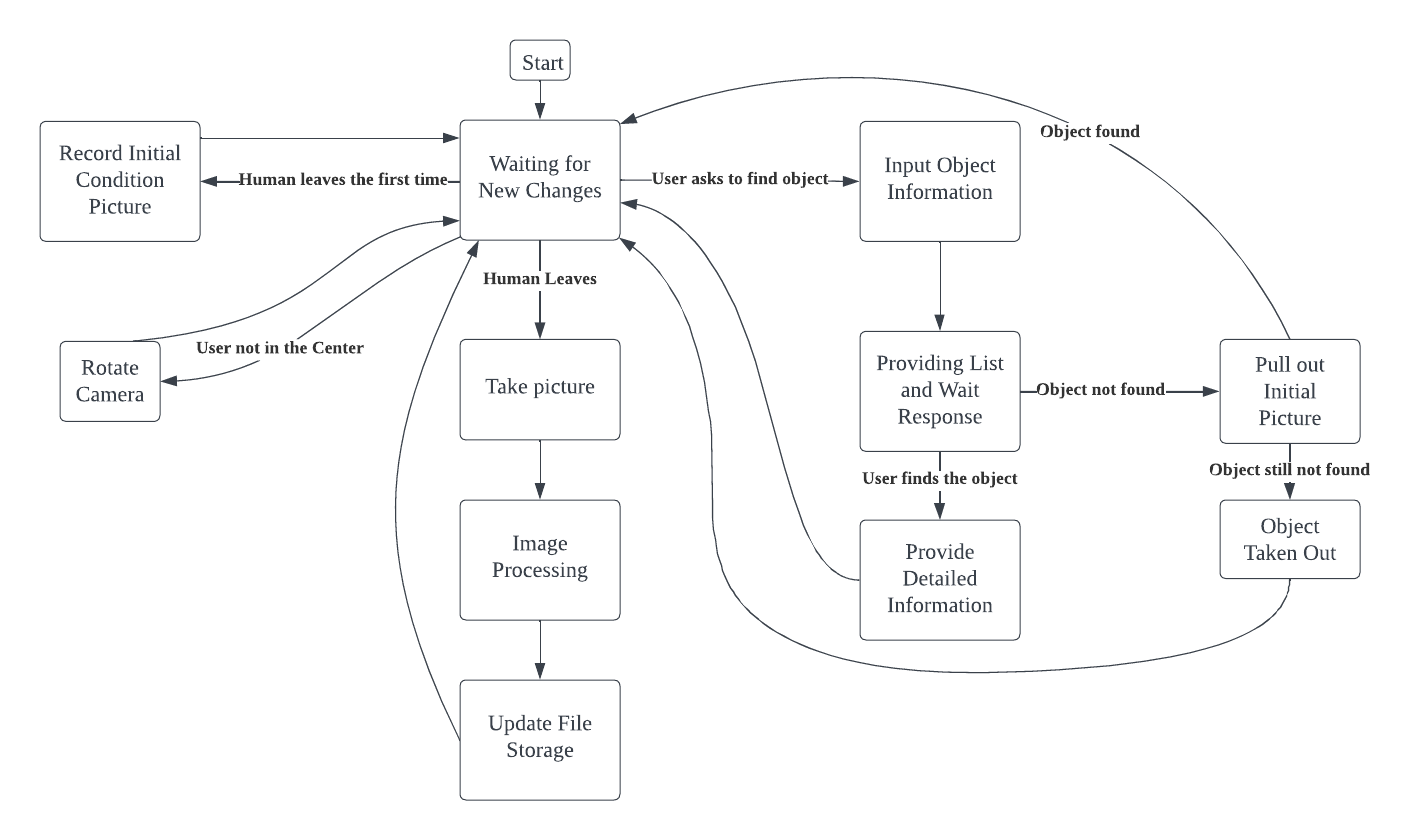
\includegraphics[scale=0.7]{FSM.png}
    \caption{The Picture of Finite  State Machine}
\end{figure}
\textbf{Record Initial Condition:} The device will take a picture of the room as the initial position information for each object and save it to the database. \\\\
\textbf{Waiting for New Changes:} The device will wait for future operations made by human or changes of objects detected by the camera. \\\\
\textbf{Detect Object Movement:} When the device detects the movement of an object that is made by another object (for example, colliding with another object and fall), it will trace the new location oof the object. \\\\
\textbf{Detect Hand Movement:} When the device detects the movement of the user, it will track the movement of the hand to identify which object is being moved and remember its final location. \\\\
\textbf{Updating:} The device will record the updated information (including time, Location, picture of object, and so on) of the object into the database.\\\\
\textbf{Input Object Information} When the user want to find one object in the room, the user interface will ask the user to input information of the object (like size, color, last time saw it, and so on).\\\\
\textbf{Providing List and Wait Response:} After the user has input the information, the system will provide a list of objects with pictures that satisfy the input information.\\\\
\textbf{Provide Detailed Information:} WHen the user find the target object, the device will display the detailed information about the object like showing the current location on the screen. \\\\
\textbf{Pull Out Initial Picture:} When the object is not found in the list, the devide will display the picture taken just after the program starts to let the user find the object.\\\\
\textbf{Object Taken Out:} If the object is still not found, the system will think that the object is taken out of the room or is hidden behind another object. \\\\
\textbf{Rotate Camera:} If the device found the human body detected is not in thhe center of the screen or the camera is covered by something else, it will send signals to the motor to rotate the camera until problem sloved. 

\subsection{Use Case Diagram}
\begin{figure}[H]
    \centering
    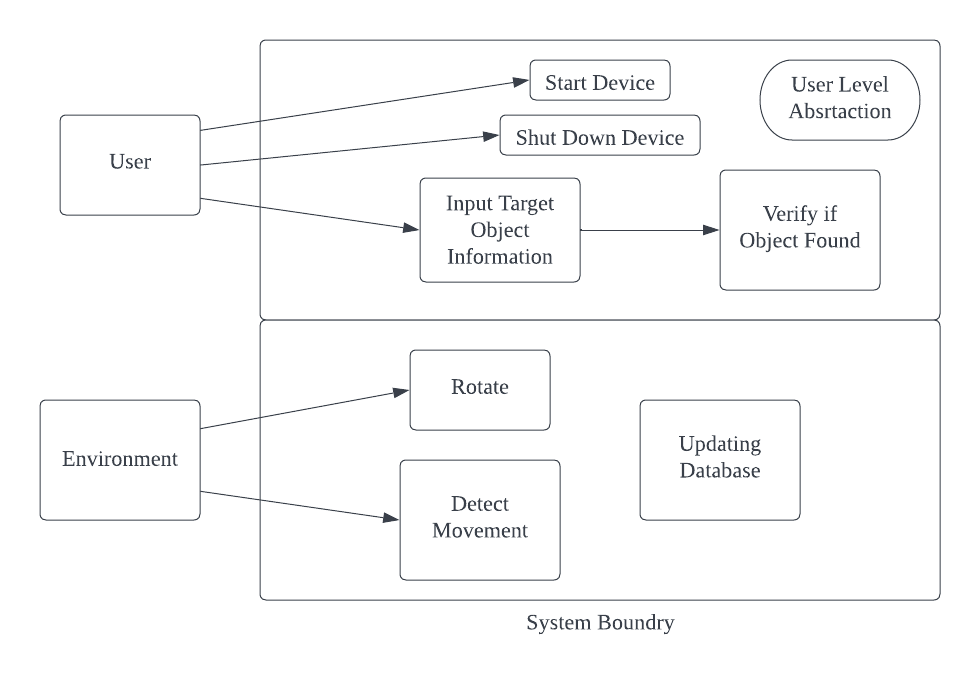
\includegraphics[scale=0.8]{Use.png}
    \caption{The Picture of Use Case Diagram}
\end{figure}
The Use Case Diagram shown above describes some actions that the user can interact with teh system. The line in the middle shows the boundaries between user and the internal program. The outmost large box shows the boundary for the whole system. All user can do is just to start and shut down the program. Th user can also find the target object by typing the information about the object and verify if the object is found. The system will interact with the environment by rotating its camera and detecting the movement of the object in the room. It will also ba able to update its database when the position of the object is changed. 

\section{Functional Requirements}
The following are the functional requirements of the project. They are separated into 2 main parts: Image Processing and Storage, and UI Interface Menu.
\subsection{Image Processing and Storage Requirements}

\textbf{IPR1:} The system should be able to identify human's body.\\\\
\textbf{Rationale:} To ensure that the movement of human’s body can be captured.\\\\
\textbf{IPR2:} The system must be able to identify human's hand.\\\\
\textbf{Rationale:} To ensure that the movement of human’s hand can be captured.\\\\
\textbf{IPR3:} The system should be able to identify all the small items being exposed to the camera.\\\\
\textbf{IPR4:} The system should be able to take a photo once the change of the location of an item is captured.\\\\
\textbf{IPR5:} The system should be able to differentiate one item from another items which are identified by the system through 3 main parameters, item\_shape, item\_color and item\_size.\\\\
\textbf{IPR6:} The system must be able to store all the photos into a file, and indicate the time when it was taken.\\\\
\textbf{IPR7:} The system must be able to name each item with a unique ID.\\\\
\textbf{IPR8:} The system should be able to arrange the photos stored in the file in ascending or descending order according to the time it was taken.\\\\
\textbf{IPR9:} The system should be able to arrange the photos stored in the file in ascending or descending order according to their IDs.

\subsection{UI Interface Menu Functional Requirements}
\textbf{UIR1:} The UI should be able to let user to choose whether to highlight a certain item or not.\\\\
\textbf{UIR2:} The UI should be able to let user to switch the ordering method.\\\\
\textbf{UIR3:} The UI must be able to notify the user when the WIFI signal is weak or unstable.\\\\

\textbf{UIR4:} The UI must be able to allow the user to view the system’s status at any given point in time.\\\\
\textbf{Rationale:} To ensure that the system will remain operational.


\section{Nonfunctional Requirements}
The next paragraphs will talk about about nonfunctional requirements in the designing of the smartVault, which will be discussed in several different parts. 
\subsection{Look and Feel Requirements}
\subsubsection{Appearance Requirements}
\textbf{APR1:} The device should not have exposed internal electronic wiring.\\\\
\textbf{APR2:} The sharp corners should not be exposed to the users annd should be covered by some soft materials.
\subsubsection{style}
Not Applicable.
\subsection{Usability and Humanity Requirements}
\subsubsection{Easy of Use Requirements}
\textbf{EUR1:} The device should be easy to installed in the room.\\\\
\textbf{EUR2:} Fonts, blanks and graphics shown on the screen should be big and visiable enough for the user to use without inserting wrong information.
\subsubsection{Personalization and Internationalization Requirements}
Not applicable.
\subsubsection{Learning Requirements}
\textbf{LR1:} The software part of the product should be easy to install.\\\\
\textbf{LR2:} The product should be easy to set up in its working environment.\\
\textbf{Rationale:} The device can identify objjects in the room in a short tiime after powering up.
\subsubsection{Understandability and Politeness Requirements}
\textbf{UPR1:} The graphics used should be readeable and visiable to the user.\\
\textbf{Rationale:} Easy for clients to find objects that wish to find in the room.
\subsection{Accessibility Requirements}
\textbf{AR1:} The display window should be concise enough for user to understand
\subsection{Performance Requirements}
\subsubsection{Speed and Latency Requirements}
\textbf{SLR1:} The response time of the product to show the location of the object should be less than 5 seconds.
\subsubsection{Safety-Critical Requirements}
\textbf{SCR1:} The base of the device should be strong enough without falling from the floor.\\\\
\textbf{SCR2:} The device should not infringe on user's privacy.\\\\
\textbf{SCR3:} The rotating speed of the motor should be slow enough without hurting people.
\subsubsection{Precision and Accuracy Requirements}
\textbf{PAR1:} The time based value used in the device should be precised to minute.\\\\
\textbf{PAR2:} The location value used in the devce should be precised to whole number.\\\\
\textbf{PAR3:} Other numatic values used in the device should be rounded to one decimal place.
\subsubsection{Reliability and Avaliability Requirements}
\textbf{RAR1:} The device should not over-rotate to an unexpected angle.\\\\
\textbf{RAR2:} The device should be avaliable to work for the whole time of except for maintaince or updating time.
\subsubsection{Robustness or Fault-Tolerance Requirements}
\textbf{RFR1:} The data stored in the file should not be deleted or changed even after the program shuts down.\\\\
\textbf{RFR2:} The device should be able to notify user for an error occurs in the program.\\
\textbf{Rationale:} The user should be notified if he or she has a wrong input or havin inappropriate actions.
\subsubsection{Capacity Requirements}
\textbf{CR1:} The device sould be able to store the any information about the location of each object detected from the camera.
\subsubsection{Scalability or extensibility Requirements}
Not applicable.
\subsubsection{Longevity Requirements}
\textbf{LR1:} The device should store the information about the objects until it is changed into a different environment.
\subsection{Operational and Environmental Requirements}
\subsubsection{Expected Physical Environment}
\textbf{EPE1:} The device is supposed to work in any indoor space.
\subsubsection{Requirements for Interfacing with Adjacent Systems}
Not applicable.
\subsubsection{Productization Requirements}
Not applicable.
\subsubsection{Release Requirements}
No applicable.
\subsection{Maintainability and Support Requirements}
\subsubsection{Maintenance Requirements}
\textbf{MR1:} The maintenance for the device should be done by the developers.
\subsubsection{Supportability Requirements}
\textbf{SR1:} The device is supported by any computers supports both C and python programming languages.
\subsubsection{Adaptability Requirements}
Not Applicable.
\subsection{Security Requirements}
\subsubsection{Access Requirements}
\textbf{AR1:} Any one except for the users is not allowed to access the any file that stores the information about the objects in the room.\\\\


\subsubsection{Integrity Requirements}
\textbf{IR1:} Data in teh files should not be changed unnecessarily.\\\\
\textbf{IR2:} The files are locked whhen teh device shuts down.
\subsubsection{Privacy Requirements}

\textbf{PR1:} Other users are not allowed to access any file in the computer.\\\\

\textbf{PR2:} The camera should only work for a specific user.
\subsubsection{Audit Requirements}
Not applicable.
\subsubsection{Immunity Requirements}
Not applicable.
\subsection{Cultural and Political Requirements}
\subsubsection{Cultural Requirements}
Not applicable.
\subsubsection{Plitical Requirements}
Not applicable.
\subsection{Legal Requirements}
\subsubsection{Compliance Requirements}
\textbf{CR1:} The performance of the product should not violate the laws that protect the privacy of thee user.
\subsubsection{Standards Requirements}
Not applicable.


\section{Traceability and Priority}
For both functional and nonfunctional requirements, the dependency matrix is made and priorities are assigned to each requirement. The Traceability matrix and priority table are shown below. In additon, the likelihood change of the requirements and the future plan of the requirements are also shown below.

\subsection{Traceability Matrix}
\begin{tabular}{|p{0.45\textwidth}| p{0.45\textwidth}|}
\hline \multicolumn{2}{|c|}{Table 1: The Table of Requirement Traceability Matrix}\\

\hline Functional Requirement ID&Nonfunctional Requirement ID\\

\hline IPR4, IPR5&LR2\\

\hline IPR8, IPR9&UPR1, PAR2\\
\hline UIR4&RFR2\\
\hline IPR6, IPR7&CR1\\
\hline

\end{tabular}

\subsection{Priority Table}
\begin{tabular}{|p{0.36\textwidth}|p{0.42\textwidth}|p{0.1\textwidth}|}

\hline \multicolumn{3}{|c|}{Table 2: The Priority Table for each Requirement}\\

\hline Functional Requirement ID&Nonfunctional Requirement ID&Priority\\

\hline IPR2, IPR3, IPR3, IPR4, IPR5, IPR6, IPR7, UIR1, UIR4&LR2, UPR1, SCR2, PAR1, PAR2, PAR3, RFR1, RFR2, CR1, EPE1, IR1, CR1&HIGH\\

\hline IPR8, IPR9, UIR2&APR1, APR2, EUR2, AR1, SCR3, RAR1, RAR2, SR1, AR1, IR2, PR1, PR2&MID\\

\hline UIR3&EUR1, LR1, SCR1, MR1&LOW\\

\hline

\end{tabular}

\subsection{Likelihood of Changes}

\begin{tabular}{|p{0.25\textwidth}|p{0.15\textwidth}|p{0.60\textwidth}|}

\hline \multicolumn{3}{|c|}{Table 3: Requirements that are Likely to Change}\\

\hline Requirement ID&Likelihood&Ways to Change\\

\hline IPR2(func)&Very Likely&The detection method of user moving the object may not just focused on the movement of hand but on other aspects.\\

\hline IPR9(func)&likely&Since time is the easiest way to track an object, the assistance information may be changed so the ordering method may also be changed.\\

\hline UIR1(func)&likely&The device will remember each object that is moved so this function may be useless.\\

\hline UIR2(func)&likely&The sorting method is determined by the program not the user, so the ording method may not depend on the user. \\

\hline EUR1(nonfunc)&likely&The physical installation of the device may be changed after the model is built.\\

\hline SCR1(nonfunc)&likely&The base may be changed when the installation method of the device changed/\\

\hline CR1(nonfunc)&very likely&The device may only choose information that make the sorting algorithm easier.\\

\hline

\end{tabular}

\subsection{Requirement Timeline}

\begin{tabular}{|p{0.5\textwidth}|p{0.5\textwidth}|}

\hline \multicolumn{2}{|c|}{Table 4: The Timeline for each Requirement}\\

\hline Requirement ID&Finish Date\\


\hline IPR1, IPR3, IPR6, AR1, PAR1, PAR2, PAR3, SR1&2022.10.31\\

\hline RFR1, CR1, AR1, IR1, PR1, PR2&2022.11.15\\

\hline IPR2, IPR4, IPR5, UIR1, UIR3, UIR4, LR2, RFR2&2022.11.28\\

\hline EUR2, SLR1, IR2&2022.12.15\\

\hline IPR7, IPR8, IPR9, UIR2, UPR1, SCR2, SCR3, RAR1&2022.12.30\\

\hline EUR1, LR1, SCR1, RAR2, EPE1, MR1, CR1&2023.1.15\\

\hline

\end{tabular}


\section{Project Issues}

\subsection{Open Issues}

\begin{itemize}
    \item Limit of 180 rotation degree of servo motor
    \item Accuracy of object detection 
    \item How to distinguish two objects with very limited resources
    \item How to recognize the same object in different angles
    \item How to guarantee the stability of the serial communication
\end{itemize}


\subsection{Off-the-Shelf Solutions}
\begin{itemize}

    \item Huskylens - is a AI camera which can learn new objects and recognize them. It has the machine learning technology enables projects to interact with people and environments which allows many kinds of system control.
    \item NVIDIA Jetson TX2 - is an embedded AI computer device. It has 8GB memory and 59.7GB/s of memory bandwidth which provides a high quality AI performance to build efficient AI models including computer vision.
\end{itemize}


\subsection{New Problems}
    \subsubsection{Effects on the Current Environment}
       \hspace{0.5cm} Any changes to the exist database may cause the data related to each object missing
    \subsubsection{Effect on the Installed Systems}
        \hspace{0.5cm} Changes to the motorized camera mount will affect the algorithm or logic of the controller board
    \subsubsection{Potential User Problems}
        \hspace{0.5cm} Changes to the user interface may change the way that user used to search the object
    
    \subsubsection{Limitations in the Anticipated Implementation Environment}
        \hspace{0.5cm}NA
    \subsubsection{Follow-Up Problems}
        \hspace{0.5cm} The changes in computer vision algorithm may cause the whole system malfunction

\subsection{Tasks}
    \subsubsection{Project Planning}
    NA
    
    \subsubsection{Planning of the Development Phases}
    NA
\subsection{Migration to the New Product}
    \subsubsection{Requirements for Migration to the New Product}
        \begin{itemize}
            \item All the objects data should be stored 
            \item Motorized camera mount should be calibrated before using
            \item The spec of camera should be kept in same as possible
        \end{itemize}
    \subsubsection{Data that Has to be Modified or translated for the new system}
        \begin{itemize}
            \item Objects data need to be transfer ed into the new system
        \end{itemize}

\subsection{Risks}
\begin{itemize}
    \item Connection lost between the board and camera during the motor movement.
    \item Inappropriate distance measure and control between the object and the motor which furthermore cause damage or stuck.
    \item Physical damage from collision with objects .
    \item Physical damage from wire twisting during rotation.
    \item Unexpected movement caused by the delay of data transfer
\end{itemize}
\subsection{Costs}
\begin{large}
\begin{center}
    \begin{tabular}{|| c || c ||}
    \hline
    Product & Price\\
    \hline\hline
    USB Camera & \$30\\
    \hline
    PTZ Mount & \$25\\
    \hline
    Arduino & \$30\\
    \hline
    Motors & \$15\\
    \hline
    Total & \$100\\
    \hline
    \end{tabular}
\end{center}
\end{large}
\subsection{User Documentation and Training}
    \subsubsection{User Documentation Requirements}
    \begin{itemize}
        \item User manuals
        \item Installation manuals
        \item Technical specifications to accompany the product
    \end{itemize}
    
    \subsubsection{Training Requirements}
    NA
\subsection{Waiting Room}
\begin{itemize}
    \item Expanding chassis's activity area including rotation angle and planar movement.
    \item Developing new algorithm regarding data transfer to enable faster real-time reaction.
    \item Adding alarm in case that object not found in the assigned area as an application of storage security.
\end{itemize}
\subsection{Ideas for Solutions}
\begin{itemize}
    \item Use DC motor with decoder to implement the unlimited rotation degree of camera mount
    \item Use Field Oriented Control algorithm to implement the unlimited rotation degree of camera mount
    \item Use frame-to-frame compassion to detect the relocation of objects
    \item Predict the possible location of objects by tracking the users path in the room
    \item Beeper alert when the camera view is not cleared
\end{itemize}




\newpage

\bibliographystyle {plainnat}
\bibliography {../../refs/References}

\newpage

\section{Appendix}

This section has been added to the Volere template.  This is where you can place
additional information.

\subsection{Symbolic Parameters}

The definition of the requirements will likely call for SYMBOLIC\_CONSTANTS.
Their values are defined in this section for easy maintenance.

\subsection{Reflection}

Our team consists of 5 mechatronics student and is developing a mechatronics system where both hardware and software components are essential for success. There are may different skills and knowledge that ties into the success of the project. Many of these required skills might new and unfamiliar to some of the group members. However, as this is a project over a span of 6 months, there are plenty of time and opportunities to pick up and master some new skills. The learning of such skills will be delegated to different team members and mastered by them before delivering and teaching others member about it.  

The project is heavily relying on a functional, reliable, and efficient software system that involve live time object detection and image processing. The coding will be done in Python, so each member needs to have adequate skill of programming in Python and able to develop and test a python program. Knowledge of image processing and object detection also should be acquired.  In order to master the skills for programming in python and image processing, team members should practice and conduct research on different object detection method. It is required for the assigned team members to compare and learn from different method and making sure that our chosen method would yield the best results given our requirements. This part of the learning is assigned to Edward, Peng and Jinhua. Edward has gained relevant knowledge through courses he took and projects he did. Peng and Jinhua have great enthusiasm for this topic and would like to conduct research on it. 

Another software component is the user interface. Members of the team should be able to build and maintain a working webpage using JavaScript. This skill is obtained by Edward through his co-op and other experiences. Erping and Jinhua also are assigned to perfect their abilities in such area. The path to success for this is to read relevant documents and tutorials, as well as practicing with small projects.
In order to communicate between the software and hardware, related programming skills are needed. Erping as the lead developer for this topic has multiple experiences and with the help of Guangwei who has exceptional skills in this field, they will be able to excel the required skills and guide other members of the team.  

On the hardware side, Guangwei will be the lead and responsible for the learning and teaching of the related skills. 3D modeling is needed for the building and 3D printing the camera mount. This skill is assigned to Guangwei and can be mastered through practicing and watching tutorials. Arduino board is the chosen board for handling the control of the motors and repositioning of the camera. Sufficient knowledge and skills to program Arduino is needed. This task is assigned to Erping and Guangwei. They both have experiences in this field and will be able to teach the rest of the team. Knowledge associated with handling motor movement is also needed and can be mastered by reviewing course notes and refreshing past knowledge. 

Aside from the hardware and software system, there are also skills associated with team management and team communication. In order to maintain a desired work plan and team coordination, it is important for all members of the team to possess the skills to work under a team environment. Members need to be comfortable and familiar with github and in order to excel, one must practice different github actions and commends. One also can improve on this by watching tutorial videos. Working in a team environment, it is important to have good communication skills and making sure people are on the same page. This can be mastered by actively engage in team meetings and ask for help when needed.  

To conclude, for a professional project like the capstone, there are many aspects to it and many skills are required. It is important to delegate different learning tasks to individual and be able to teach the new skillset to the rest of the team. The following are the skills mentioned in previous paragraphs and is the overview of the assignment of the learning process:


\begin{enumerate}
  \item communication and team management (All)
  \item Github (All)
  \item Python, image processing and object detection (Edward, Jinhua, Peng)
  \item Arduino and control (Erping and Guangwei)
  \item Motor control (Erping and Guangwei)
  \item Javascript (Edward, Peng, Jinhua)
  \item 3D modeling and 3D printing (Erping and Guangwei)
  \item Writing and presenting reports (All)
\end{enumerate}

\end{document}
